\documentclass[aspectratio=169,12pt,t]{beamer}

% --- Theme: Metropolis (modern, clean) ---
\usetheme[progressbar=frametitle,numbering=fraction,block=fill]{metropolis}

% --- Fira Sans font (install texlive-fonts-extra if missing) ---
\IfFileExists{FiraSans.sty}{\usepackage[sfdefault]{FiraSans}}{}

% --- Light background with warm accent ---
\definecolor{mDarkTeal}{RGB}{35,55,59}
\definecolor{mLightBrown}{RGB}{235,228,216}
\definecolor{mAccent}{RGB}{140,70,20}

\setbeamercolor{normal text}{fg=mDarkTeal,bg=white}
\setbeamercolor{alerted text}{fg=mAccent}
\setbeamercolor{frametitle}{bg=mDarkTeal,fg=white}
\setbeamercolor{progress bar}{fg=mAccent,bg=mLightBrown}
\setbeamercolor{title separator}{fg=mAccent}
\setbeamercolor{progress bar in head/foot}{fg=mAccent,bg=mLightBrown}
\setbeamercolor{progress bar in section page}{fg=mAccent,bg=mLightBrown}

% --- Packages ---
\usepackage[utf8]{inputenc}
\usepackage{amsmath,amssymb,amsthm}
\usepackage{mathrsfs}
\usepackage{tikz}
\usetikzlibrary{arrows.meta,positioning,calc,decorations.pathreplacing,shapes,patterns}
\usepackage{pgfplots}
\pgfplotsset{compat=1.18}

% --- Custom colors for content types ---
\definecolor{defcolor}{RGB}{25,85,120}
\definecolor{thmcolor}{RGB}{140,35,35}
\definecolor{proofcolor}{RGB}{35,100,50}
\definecolor{excolor}{RGB}{140,75,10}
\definecolor{remcolor}{RGB}{90,90,90}

% --- Beamer blocks for mathematical content types ---
\newenvironment{defblock}[1]{%
  \setbeamercolor{block title}{bg=defcolor,fg=white}%
  \setbeamercolor{block body}{bg=defcolor!5}%
  \begin{block}{#1}}{\end{block}}

\newenvironment{thmblock}[1]{%
  \setbeamercolor{block title}{bg=thmcolor,fg=white}%
  \setbeamercolor{block body}{bg=thmcolor!5}%
  \begin{block}{#1}}{\end{block}}

\newenvironment{proofblock}[1]{%
  \setbeamercolor{block title}{bg=proofcolor,fg=white}%
  \setbeamercolor{block body}{bg=proofcolor!5}%
  \begin{block}{#1}}{\end{block}}

\newenvironment{exblock}[1]{%
  \setbeamercolor{block title}{bg=excolor,fg=white}%
  \setbeamercolor{block body}{bg=excolor!5}%
  \begin{block}{#1}}{\end{block}}

\newenvironment{remblock}[1]{%
  \setbeamercolor{block title}{bg=remcolor,fg=white}%
  \setbeamercolor{block body}{bg=remcolor!5}%
  \begin{block}{#1}}{\end{block}}

% --- Metadata ---
\title{Chapter 1: The Real and Complex Number Systems}
\subtitle{Section: The Extended Real Number System}
\author{Based on Walter Rudin's \emph{Principles of Mathematical Analysis}}
\date{}

\begin{document}

% =============================================================================
% TITLE AND OUTLINE
% =============================================================================

\begin{frame}
  \titlepage
  \note{
    Welcome to Chapter 1, Section 5: The Extended Real Number System.
    This is a short but important section where we extend the real numbers
    by adding two new symbols: plus infinity and minus infinity. This
    extension is not about creating new ``numbers'' in the algebraic sense,
    but about providing a convenient framework so that expressions like
    the supremum of an unbounded set always make sense.
  }
\end{frame}

\begin{frame}{Outline}
  \tableofcontents
  \note{
    Here is our outline for this section. We will start with the motivation
    for extending the real number system, then state the formal definition,
    look at a diagram of the extended real line, discuss the consequences
    for suprema and infima, go through the arithmetic conventions, and
    wrap up with a summary.
  }
\end{frame}

% =============================================================================
% MOTIVATION
% =============================================================================

\section{Motivation}

% --- Build 1/3 ---
\begin{frame}{Why Extend the Real Numbers?}
  \begin{itemize}
    \item In $\mathbb{R}$, unbounded sets have \emph{no} supremum or infimum
  \end{itemize}

  \note{
    Before we state the definition, let's understand why this extension is
    useful. In the real number system, if a set is not bounded above, then
    it simply has no supremum. For example, the set of all positive integers
    has no least upper bound in the reals. This is inconvenient because we
    often want to write expressions involving suprema without first checking
    whether the set is bounded. So what do we really want?
  }
\end{frame}

% --- Build 2/3 ---
\begin{frame}{Why Extend the Real Numbers?}
  \begin{itemize}
    \item In $\mathbb{R}$, unbounded sets have \emph{no} supremum or infimum
    \item We want $\sup E$ and $\inf E$ to \alert{always exist} for nonempty $E$
  \end{itemize}

  \note{
    The goal is to set up a system where every nonempty subset has both
    a least upper bound and a greatest lower bound. This makes many
    statements in analysis cleaner and avoids endless case distinctions
    about whether a set is bounded or not. How can we achieve this?
  }
\end{frame}

% --- Build 3/3 ---
\begin{frame}{Why Extend the Real Numbers?}
  \begin{itemize}
    \item In $\mathbb{R}$, unbounded sets have \emph{no} supremum or infimum
    \item We want $\sup E$ and $\inf E$ to \alert{always exist} for nonempty $E$
    \item Solution: add two symbols, $+\infty$ and $-\infty$, to the real line
  \end{itemize}

  \note{
    The solution is elegant and simple: we adjoin two new symbols, plus
    infinity and minus infinity, to the real line. These are not real
    numbers and do not obey all the field axioms, but they give us a
    convenient extended system. Let's see the formal definition.
  }
\end{frame}

% =============================================================================
% DEFINITION
% =============================================================================

\section{Definition}

\begin{frame}{Definition 1.23: The Extended Real Number System}
  \begin{defblock}{Definition 1.23}
    The \alert{extended real number system} consists of the real field $\mathbb{R}$
    together with two symbols, $+\infty$ and $-\infty$, subject to the ordering:
    \[
      -\infty \;<\; x \;<\; +\infty \quad \text{for every } x \in \mathbb{R}.
    \]
  \end{defblock}

  \vspace{0.5em}
  The original order among real numbers is preserved.

  \note{
    Here is Definition 1.23. The extended real number system is the real
    field "R" together with two new symbols: plus infinity and minus infinity.
    We keep the original ordering among the real numbers exactly as before,
    and we declare that minus infinity is less than every real number, and
    every real number is less than plus infinity. So minus infinity is the
    smallest element and plus infinity is the largest element in this
    extended system.
  }
\end{frame}

% --- Diagram: the extended real line ---
\begin{frame}{The Extended Real Line}
  \begin{center}
  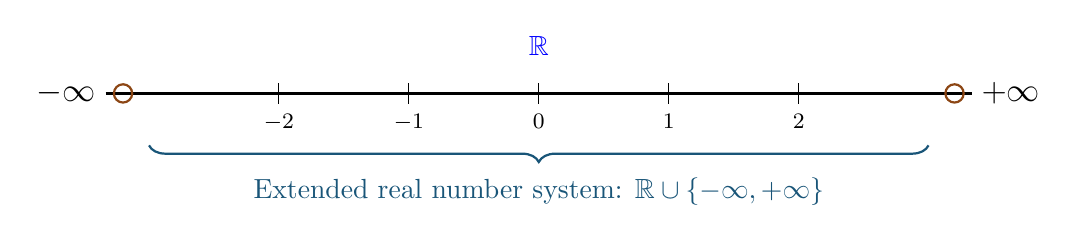
\begin{tikzpicture}[scale=1.1]
    % Main real line
    \draw[thick] (-5,0) -- (5,0);

    % Infinity symbols at ends
    \node[left] at (-5,0) {\large $-\infty$};
    \node[right] at (5,0) {\large $+\infty$};

    % Open circles at infinities (not real numbers)
    \draw[thick, mAccent] (-4.8,0) circle (3pt);
    \draw[thick, mAccent] (4.8,0) circle (3pt);

    % Tick marks for reference points
    \foreach \x/\lab in {-3/-2, -1.5/-1, 0/0, 1.5/1, 3/2} {
      \draw (\x, -0.12) -- (\x, 0.12);
      \node[below=4pt] at (\x,0) {\footnotesize $\lab$};
    }

    % Label the real line
    \node[blue, above=10pt] at (0,0) {$\mathbb{R}$};

    % Braces and labels
    \draw[decorate, decoration={brace, amplitude=6pt, mirror}, thick, defcolor]
      (-4.5,-0.6) -- (4.5,-0.6)
      node[midway, below=8pt, defcolor] {Extended real number system: $\mathbb{R} \cup \{-\infty, +\infty\}$};
  \end{tikzpicture}
  \end{center}

  \vspace{0.3em}
  \begin{itemize}
    \item Open circles: $+\infty$ and $-\infty$ are \emph{not} real numbers
    \item They are \emph{symbols} adjoined to $\mathbb{R}$ with a defined ordering
  \end{itemize}

  \note{
    This diagram shows the extended real line. The real numbers sit in the
    middle, just as before. At the far left we have minus infinity and at
    the far right we have plus infinity, shown with open circles to
    emphasize that these are not actual real numbers. They are symbols
    that we adjoin to the real line purely for convenience. The key point
    is that the ordering is total: every element is comparable to every
    other element.
  }
\end{frame}

% =============================================================================
% CONSEQUENCES FOR SUPREMA AND INFIMA
% =============================================================================

\section{Consequences for Suprema and Infima}

% --- Build 1/4 ---
\begin{frame}{Suprema and Infima Always Exist}
  \begin{itemize}
    \item $+\infty$ is an upper bound of \emph{every} subset of the extended reals
  \end{itemize}

  \note{
    Now let's see the immediate payoff of this extension. Since plus infinity
    is greater than every real number and also greater than minus infinity,
    it is an upper bound of every subset of the extended real number system.
    What does that imply?
  }
\end{frame}

% --- Build 2/4 ---
\begin{frame}{Suprema and Infima Always Exist}
  \begin{itemize}
    \item $+\infty$ is an upper bound of \emph{every} subset of the extended reals
    \item Therefore: every nonempty subset has a \alert{least upper bound}
  \end{itemize}

  \note{
    Because plus infinity serves as a universal upper bound, every nonempty
    subset is guaranteed to be bounded above, and hence has a least upper
    bound in the extended system. This is a powerful simplification: we
    never have to check boundedness before taking a supremum. And of course,
    the same idea works in the other direction as well.
  }
\end{frame}

% --- Build 3/4 ---
\begin{frame}{Suprema and Infima Always Exist}
  \begin{itemize}
    \item $+\infty$ is an upper bound of \emph{every} subset of the extended reals
    \item Therefore: every nonempty subset has a \alert{least upper bound}
    \item Dually: $-\infty$ is a lower bound of every subset, so every nonempty subset has a \alert{greatest lower bound}
  \end{itemize}

  \note{
    By exactly the same reasoning, minus infinity is a lower bound of every
    subset. So every nonempty subset also has a greatest lower bound, or
    infimum. Together, these two facts mean that suprema and infima always
    exist in the extended real number system. Let's see what this looks like
    in a concrete example.
  }
\end{frame}

% --- Build 4/4 ---
\begin{frame}{Suprema and Infima Always Exist}
  \begin{itemize}
    \item $+\infty$ is an upper bound of \emph{every} subset of the extended reals
    \item Therefore: every nonempty subset has a \alert{least upper bound}
    \item Dually: $-\infty$ is a lower bound of every subset, so every nonempty subset has a \alert{greatest lower bound}
  \end{itemize}

  \vspace{0.5em}
  \textbf{Key example:} If $E \subset \mathbb{R}$ is nonempty and not bounded above in~$\mathbb{R}$, then
  \[
    \sup E = +\infty
  \]
  in the extended real number system. Similarly, $\inf E = -\infty$ if $E$ is not bounded below.

  \note{
    Here is the key example. Suppose "E" is a nonempty set of real numbers
    that is not bounded above in "R". In the ordinary real number system,
    the supremum simply does not exist. But in the extended system, we
    simply say the supremum of "E" is plus infinity. Similarly, if "E" is
    not bounded below, then the infimum of "E" is minus infinity. This
    convention lets us write suprema and infima without ever worrying
    about boundedness. Now let's turn to the arithmetic conventions for
    the extended reals.
  }
\end{frame}

% =============================================================================
% ARITHMETIC CONVENTIONS
% =============================================================================

\section{Arithmetic Conventions}

\begin{frame}{Not a Field}
  \begin{remblock}{Remark}
    The extended real number system does \alert{not} form a field.
  \end{remblock}

  \vspace{0.5em}
  Expressions like $\infty - \infty$, $\;0 \cdot \infty$, $\;\frac{\infty}{\infty}$
  are \textbf{not defined}.

  \vspace{0.5em}
  However, certain arithmetic operations \emph{are} defined by convention.

  \note{
    Before we list the arithmetic conventions, an important warning: the
    extended real number system is not a field. You cannot do arbitrary
    arithmetic with plus and minus infinity. Expressions like infinity
    minus infinity, zero times infinity, or infinity divided by infinity
    are left undefined. They are indeterminate forms that you may
    have encountered in calculus. Despite this, there are several
    useful conventions for operations that do make sense. Let's go
    through them one by one.
  }
\end{frame}

% --- Convention (a): Build 1/3 ---
\begin{frame}{Arithmetic Conventions for the Extended Reals}
  For any \emph{real} number $x$:

  \vspace{0.5em}
  \begin{defblock}{Convention (a): Addition and Division}
    \[
      x + \infty = +\infty, \qquad x - \infty = -\infty, \qquad
      \frac{x}{+\infty} = \frac{x}{-\infty} = 0.
    \]
  \end{defblock}

  \note{
    Convention "a" applies when "x" is any real number. Adding plus infinity
    to "x" gives plus infinity; subtracting infinity from "x" gives minus
    infinity. And dividing any real number "x" by plus or minus infinity
    gives zero. These make intuitive sense: no finite number can affect
    infinity by addition, and dividing a finite quantity by something
    infinitely large gives zero. Next, let's see what happens with
    multiplication.
  }
\end{frame}

% --- Convention (b): Build 2/3 ---
\begin{frame}{Arithmetic Conventions for the Extended Reals}
  For any \emph{real} number $x$:

  \vspace{0.5em}
  \begin{defblock}{Convention (a): Addition and Division}
    \[
      x + \infty = +\infty, \qquad x - \infty = -\infty, \qquad
      \frac{x}{+\infty} = \frac{x}{-\infty} = 0.
    \]
  \end{defblock}

  \vspace{0.3em}
  \begin{defblock}{Convention (b): Positive $\times$ Infinity}
    If $x > 0$: \quad $x \cdot (+\infty) = +\infty$, \quad $x \cdot (-\infty) = -\infty$.
  \end{defblock}

  \note{
    Convention "b" tells us what happens when we multiply a positive real
    number by infinity. A positive number times plus infinity is plus
    infinity, and a positive number times minus infinity is minus infinity.
    The sign is preserved because a positive scaling factor does not
    change direction. What if "x" is negative instead?
  }
\end{frame}

% --- Convention (c): Build 3/3 ---
\begin{frame}{Arithmetic Conventions for the Extended Reals}
  For any \emph{real} number $x$:

  \vspace{0.5em}
  \begin{defblock}{Convention (a): Addition and Division}
    \[
      x + \infty = +\infty, \qquad x - \infty = -\infty, \qquad
      \frac{x}{+\infty} = \frac{x}{-\infty} = 0.
    \]
  \end{defblock}

  \vspace{0.3em}
  \begin{defblock}{Convention (b): Positive $\times$ Infinity}
    If $x > 0$: \quad $x \cdot (+\infty) = +\infty$, \quad $x \cdot (-\infty) = -\infty$.
  \end{defblock}

  \vspace{0.3em}
  \begin{defblock}{Convention (c): Negative $\times$ Infinity}
    If $x < 0$: \quad $x \cdot (+\infty) = -\infty$, \quad $x \cdot (-\infty) = +\infty$.
  \end{defblock}

  \note{
    Convention "c" handles the case when "x" is negative. A negative number
    times plus infinity is minus infinity, and a negative number times
    minus infinity is plus infinity. The sign flips, just as it does
    for ordinary multiplication by a negative number. Notice that the
    case "x" equals zero is deliberately excluded from both "b" and "c".
    The expression zero times infinity is undefined, as it is an
    indeterminate form.
  }
\end{frame}

% =============================================================================
% TERMINOLOGY
% =============================================================================

\section{Terminology}

\begin{frame}{Finite vs.\ Infinite}
  \begin{remblock}{Remark: Terminology}
    When we wish to emphasize that a number $x$ belongs to $\mathbb{R}$
    (as opposed to being $+\infty$ or $-\infty$), we call $x$ \alert{finite}.
  \end{remblock}

  \vspace{1em}
  \begin{center}
  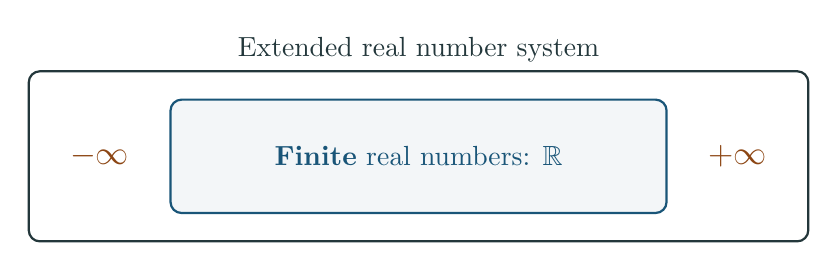
\begin{tikzpicture}[scale=0.9]
    % Box for extended reals
    \draw[thick, rounded corners, mDarkTeal] (-5.5,-1.2) rectangle (5.5,1.2);
    \node[mDarkTeal, above] at (0,1.2) {Extended real number system};

    % Box for R
    \draw[thick, rounded corners, defcolor, fill=defcolor!5] (-3.5,-0.8) rectangle (3.5,0.8);
    \node[defcolor] at (0,0) {\textbf{Finite} real numbers: $\mathbb{R}$};

    % Infinity symbols outside R but inside extended
    \node[mAccent, font=\large\bfseries] at (-4.5,0) {$-\infty$};
    \node[mAccent, font=\large\bfseries] at (4.5,0) {$+\infty$};
  \end{tikzpicture}
  \end{center}

  \note{
    Before we wrap up, a quick note on terminology. When we want to
    distinguish ordinary real numbers from plus or minus infinity, we call
    the real numbers ``finite.'' So saying ``"x" is finite'' simply means "x"
    belongs to "R". The diagram shows this: the extended real number system
    is the big box containing both the finite reals in the middle and the
    two infinite symbols on the outside. You will see this terminology
    used frequently throughout the rest of the book. Now let's summarize
    what we have learned.
  }
\end{frame}

% =============================================================================
% SUMMARY
% =============================================================================

\section{Summary}

% --- Build 1/4 ---
\begin{frame}{Summary}
  \textbf{Key takeaways:}
  \begin{itemize}
    \item The extended real number system is $\mathbb{R} \cup \{-\infty, +\infty\}$
  \end{itemize}

  \note{
    Let's review the key points from this section. First, the extended
    real number system is simply the real numbers together with two
    adjoined symbols, plus infinity and minus infinity. The ordering
    places minus infinity below everything and plus infinity above
    everything.
  }
\end{frame}

% --- Build 2/4 ---
\begin{frame}{Summary}
  \textbf{Key takeaways:}
  \begin{itemize}
    \item The extended real number system is $\mathbb{R} \cup \{-\infty, +\infty\}$
    \item Every nonempty subset has a supremum and an infimum
  \end{itemize}

  \note{
    The main benefit is that every nonempty subset now has both a least
    upper bound and a greatest lower bound. We never have to worry about
    boundedness when writing suprema or infima. This is the whole reason
    we introduced the extension.
  }
\end{frame}

% --- Build 3/4 ---
\begin{frame}{Summary}
  \textbf{Key takeaways:}
  \begin{itemize}
    \item The extended real number system is $\mathbb{R} \cup \{-\infty, +\infty\}$
    \item Every nonempty subset has a supremum and an infimum
    \item It is \emph{not} a field --- certain operations are undefined
  \end{itemize}

  \note{
    However, this convenience comes with a caveat. The extended system is
    not a field. We cannot do arbitrary arithmetic with plus and minus
    infinity. Expressions like infinity minus infinity, zero times infinity,
    and infinity divided by infinity are left deliberately undefined because
    they are indeterminate forms.
  }
\end{frame}

% --- Build 4/4 ---
\begin{frame}{Summary}
  \textbf{Key takeaways:}
  \begin{itemize}
    \item The extended real number system is $\mathbb{R} \cup \{-\infty, +\infty\}$
    \item Every nonempty subset has a supremum and an infimum
    \item It is \emph{not} a field --- certain operations are undefined
    \item Arithmetic with $\pm\infty$ follows conventions (a), (b), (c)
  \end{itemize}

  \vspace{1em}
  \textbf{Coming up next:} The Complex Field --- extending $\mathbb{R}$ in a
  completely different direction.

  \note{
    Finally, we have the three arithmetic conventions for combining real
    numbers with infinity. These will be used throughout the book whenever
    we work with limits, suprema, infima, and series. In the next section,
    we will extend the real numbers in a completely different direction:
    instead of adding infinite elements, we will add a square root of
    negative one and build the complex number field.
  }
\end{frame}

\end{document}
